% !Mode:: "TeX:UTF-8"
% !TEX program = xelatex
\documentclass{beamer}
\usetheme{AnnArbor}
%\usecolortheme{orchid}
\usepackage[UTF8,noindent]{ctexcap}
\usepackage{amsmath}
\usepackage{cases}
\usepackage{enumerate}
\usepackage{subfig}
\usepackage{tikz}
\newcommand{\Step}[1]{\textbf{Step#1}}
\graphicspath{{../thesis/figures/}}
\title{多品种装配车间调度研究}
\subtitle{论文答辩}
\author{陈晟恺}
\institute[diufanshu@gmail.com]{健行理工1001~~201002750102\\ 指导老师:鲁建厦、董巧英 }
\date{\today}
\begin{document}
\newtheorem{thm}{定理}
\begin{frame}
\titlepage
\transboxout<1->
\end{frame}
\section{绪论}
\subsection{课题研究的背景、意义及内容}
\begin{frame}{研究背景及意义}{多品种生产方式出现}
\begin{itemize}[<+-| alert@+>]
\item 同步装配流水线方式作业是现在汽车装配的主要方式。
\item 技术革新,客户需求的多样化,以及精益思想、环保节能观念的出现,汽车工业的生产模式转变为面向订单的大批量、多品种的生产方式。
\item 为配合汽车生产,汽车电子部件的装配生产也要呈现多品种与批量化。
\item 合理安排装配产线,优化调度作业单元,对保证汽车零部件装配质量,快速响应需求,提高汽车零部件装配线的生产效率有着重要的现实意义。
\end{itemize}
\transboxout<1->\end{frame}

\begin{frame}{研究技术路线}
\begin{figure}
\centering
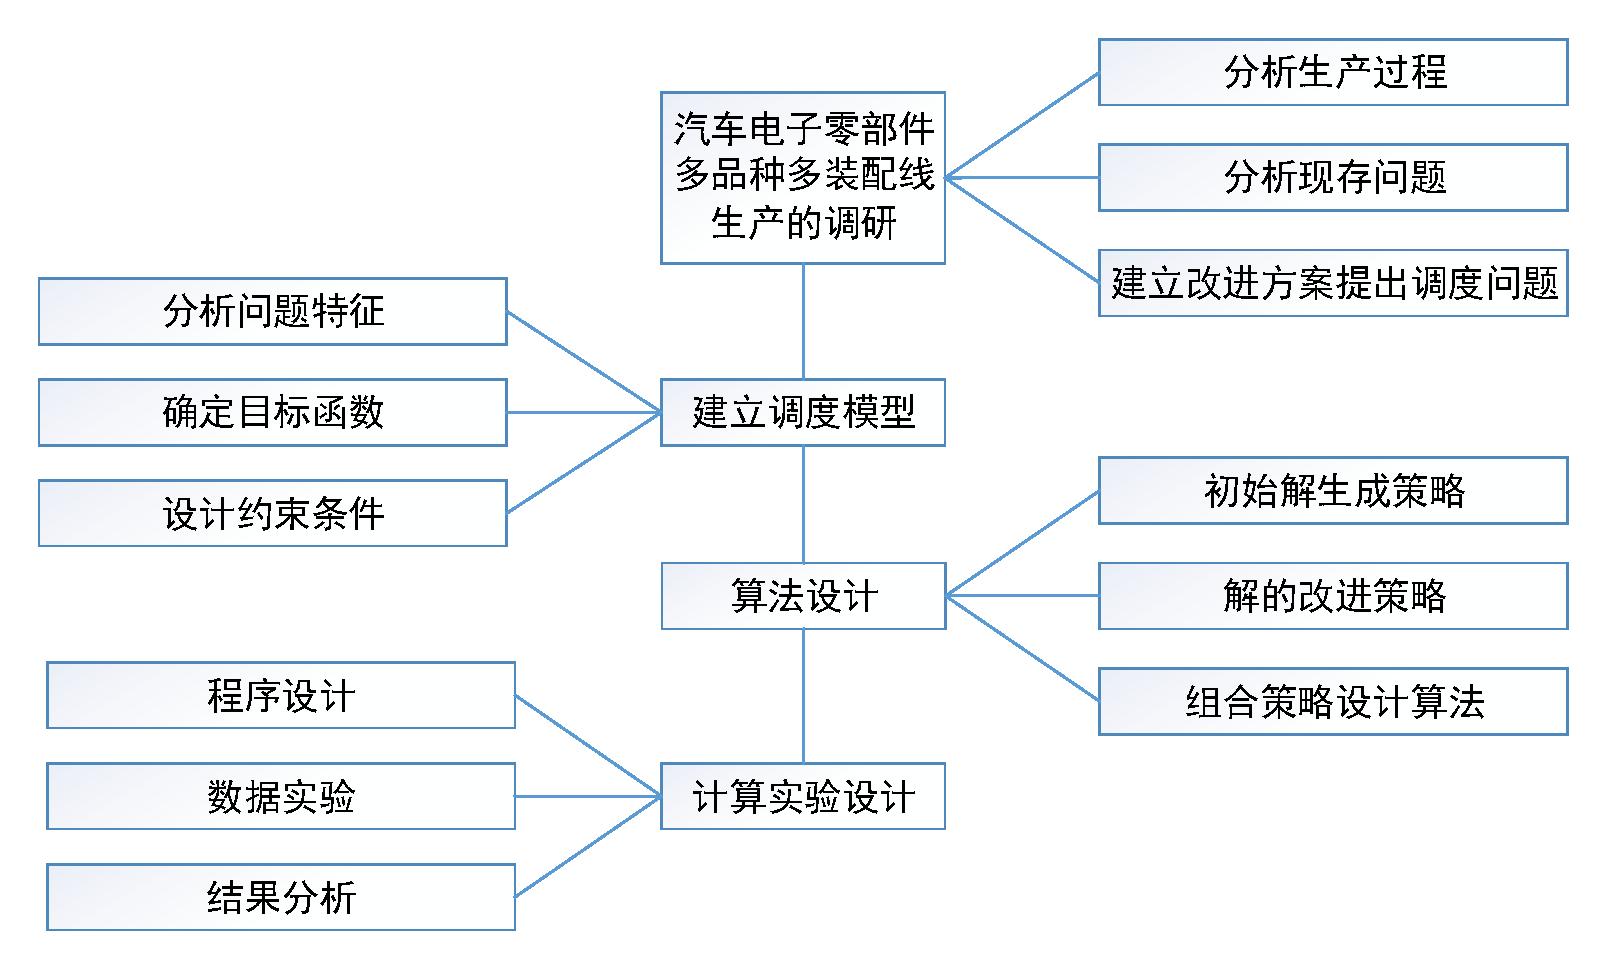
\includegraphics[width = 10cm]{techroute1.pdf}
\caption{课题研究关键技术路线}
\end{figure}
\transboxout<1->\end{frame}

\section{研究对象现状与分析}
\subsection{研究对象现状}
%\begin{frame}{公司基本情况}
%\begin{itemize}[<+-| alert@+>]
%\item 该汽车电子有限公司主要产品为车用电子电器开关、控制模块、控制面板等,是国内外 40 余家汽车主机厂的专业定点配套供应商,配套的产品型号达 6000 余种。
%\item 订单特点是品种多、批量大、小型产品、工艺成熟,所以采用流水线生产是比较合适的,与
%其合作较多的客户 (主机厂) 一般有其专用线,专门负责该主机厂的订单生产。
%\end{itemize}
%\transboxout<1->\end{frame}
\begin{frame}{装配车间现状}
\onslide<1->{采用专线生产的方式,当同
一客户有多个订单下达时,按照先到先服务 (FCFS) 的规则进行装配生产安排,多条产线并行作业互不干扰。}
\onslide<2>{\begin{figure}
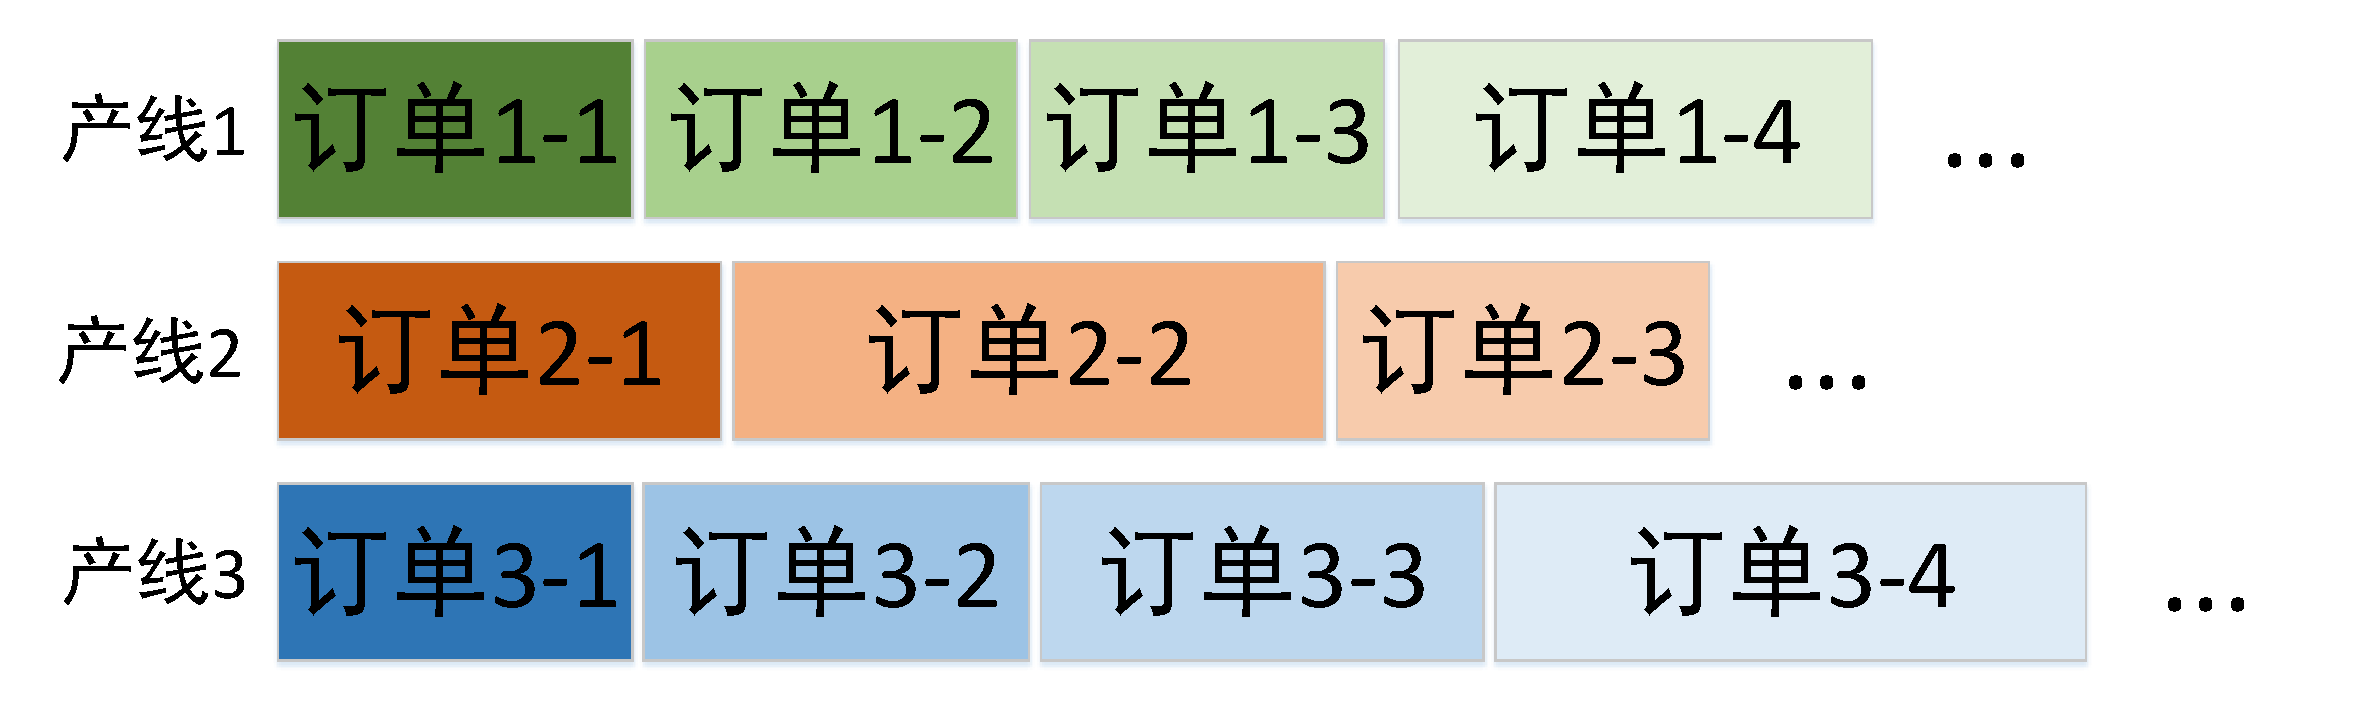
\includegraphics[width = 10cm]{orderschedulenow.pdf}
\caption{$3$条生产线的现行调度\footnote{其中订单a -- b 表示主机厂a 的第b 个订单,下同。}}
\end{figure}}
\transboxout<1->\end{frame}
\subsection{问题分析与解决思路}
\begin{frame}{装配车间分析}{存在问题}
现行调度方案存在一些改进空间,例如多条装配线负荷不均衡,有的任务过
重,有的任务不足,负荷不均衡,一条装配线上装配的产品工艺相似性较低,导致换线时间增加,产生更长
的等待。其主要问题如下:
\begin{itemize}[<+-| alert@+>]
\item 产线利用率低
\item 生产不够均衡
\item 产线冗余度高
\item 工期可控性底
\item 工艺及设备和生产需求不匹配
\end{itemize}
\transboxout<1->\end{frame}
\begin{frame}{装配车间分析}{改进设计}
\onslide<1->{目前的生产现状的主要问题是各主机厂有其专用流水线,使得订单的调度安排为较为单一,受到一些限制,不能很合理地利用流水线的生产能力,所以首要的改进是突破专用线的生产界限。如此一来,生产线可以加工多家主机厂的订单,形成所谓的混线生产。}
\onslide<2>{\begin{figure}
\centering
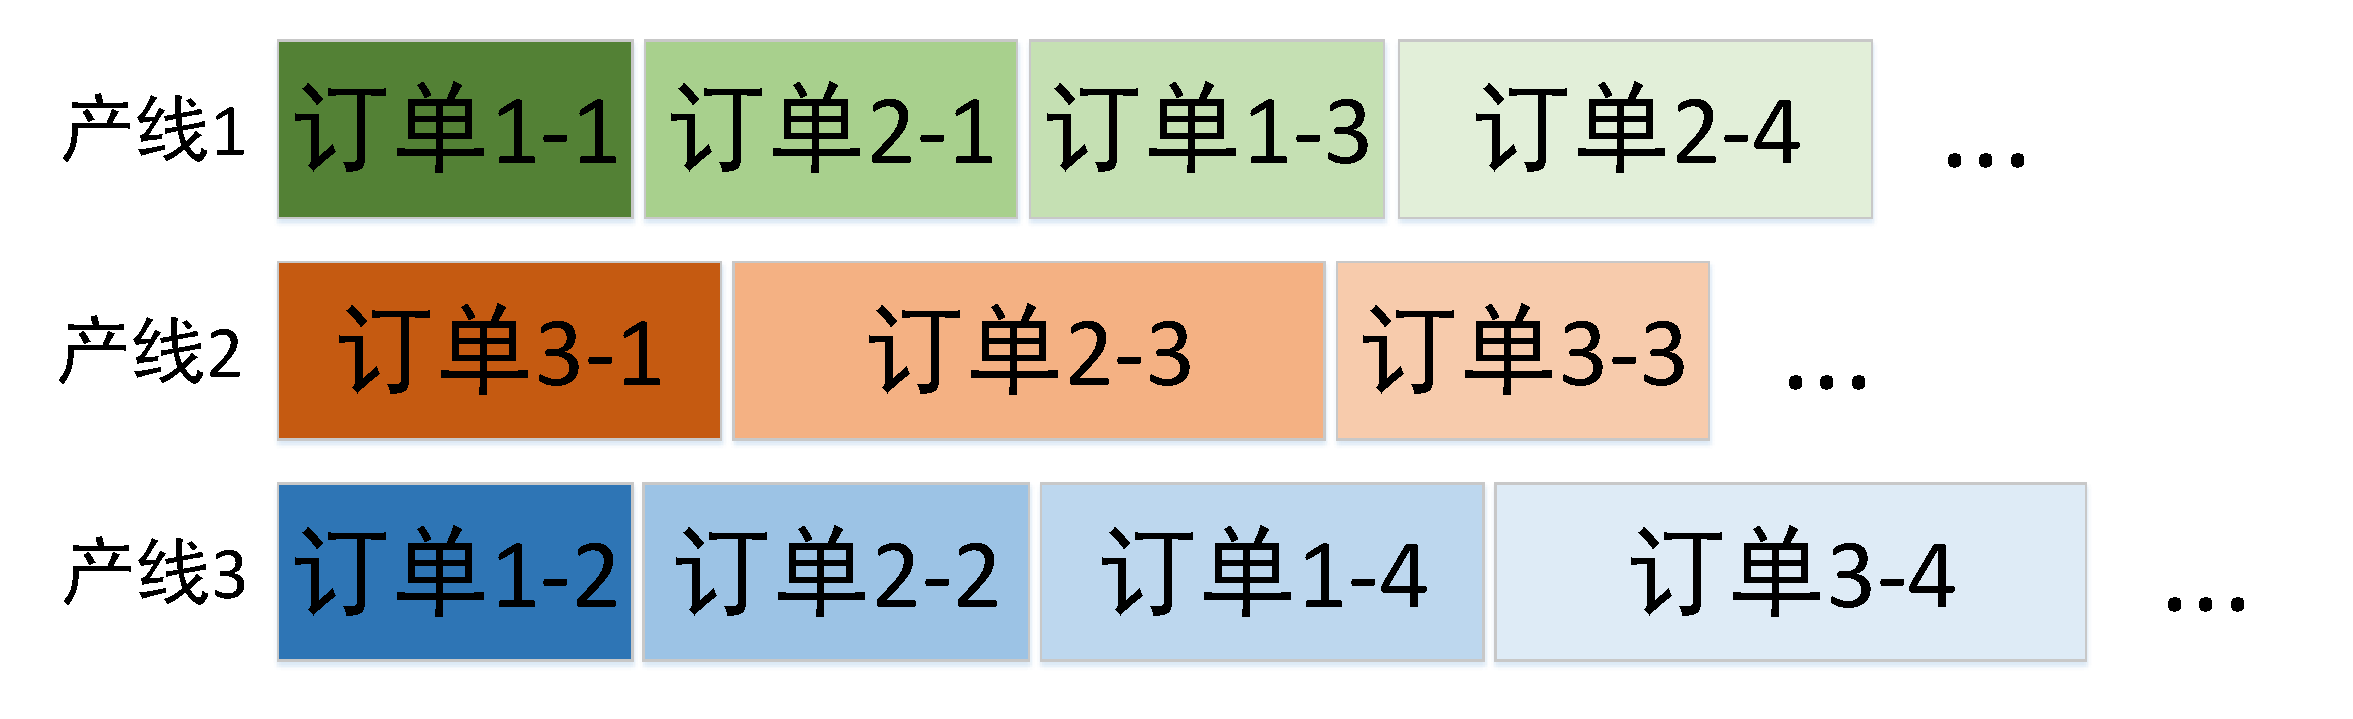
\includegraphics[width = 10cm]{oredrschedule.pdf}
\caption{$3$条产线的混线装配生产示意}
\end{figure}}
\transboxout<1->\end{frame}

\section{多品种装配车间调度建模}
\subsection{多品种多装配线轮番装配调度优化模型}
\begin{frame}{模型1}{基本假设}
\begin{itemize}[<+-| alert@+>]
\item 整数变量假设
\item 数量有限假设
\item 无差别假设
\item 无插单生产假设
\item 不可中断假设
\item 无相关假设
\end{itemize}
\transboxout<1->\end{frame}

\begin{frame}
\tiny
\begin{equation}
\min\quad \lambda_t\sum_{l=1}^m\sum_{k=1}^{|S_l|} wt_{l_k}T_{l_k} + \lambda_c\sum_{l=1}^m\sum_{k=1}^{|S_l|}wc_{l_k}C_{l_k}
\end{equation}
\begin{numcases}{s.t.}
\sum_{l=1}^m |S_l| = n\label{equ:basicst1}\\
\bigcup_{l=1}^m \overline{S_l} = N\label{equ:basicst2}\\
\sum_{l=1}^m\sum_{k=1}^{|S_l|} wt_{l_k}= 1\\
\sum_{l=1}^m\sum_{k=1}^{|S_l|} wc_{l_k}= 1\\
\lambda_c + \lambda_t = 1\\
 C_{l_1} = p_{l_1} & $l = 1,2,...,m$\label{equ:basicst3}\\
 C_{l_k} = C_{l_{k-1}} + p_{l_k} & $k = 2,3,...,|S_l|, l = 1,2,...,m$\label{equ:basicst4}\\
 p_{l_k} = p'_{l_k} + s_{l_k} & $k = 1,2,...,|S_l|, l = 1,2,...,m$\label{equ:basicst5}\\
 T_{l_k} = \max\{0, C_{l_k} - d_{l_k}\} & $k = 1,2,...,|S_l|, l = 1,2,...,m$\label{equ:basicst6}\\
 p'_{l_k}, s_{l_k}, d_{l_k}, wt_{l_k}, \lambda_t, \lambda_c\ge 0 & $k = 1,2,...,|S_l|, l = 1,2,...,m$\label{equ:basicst7}
\end{numcases}
\transboxout<1->\end{frame}

\begin{frame}{模型2}{相关假设}
\begin{itemize}[<+-| alert@+>]
\item 插单假设
\item 惩罚一致假设
\item 订单最早可处理时刻假设
\end{itemize}
\transboxout<1->\end{frame}

\begin{frame}{模型2}{相关定义}
\only<1>{\begin{block}{产线均衡率}
考虑订单陆续到达时,更为注重订单的按时交付,同时也关注流水线的生产均衡性。生产均衡性指的是
流水线的使用均衡,不要出现某条流水线一直繁忙而有些流水线空闲居多,导致负荷不均衡,损失产能。产线均衡率定义如下:
\[
Rb = \frac{\sum_{l=1}^m C_l}{\displaystyle m\times \max_{1 \le l \le m} \{C_l\}}
\]
\end{block}}
\only<2>{\begin{block}{产线的利用率}
各流水线除了切换准备,其余时间都在处理订单,在模型 2 中,流水线上订单间的空闲等待将会出现,其中切换准备同样不计入空
闲,流水线利用率定义为:
\[
Ru_l = 1 - \frac{\sum_{k=1}^{|S_l|}f_{l_k}}{C_l}
\]
其中,$f_{l_k}$为订单的闲置,定义为:
\begin{subnumcases}{f_{l_k} = }
\max\{r_{l_k} - s_{l_k}, 0\} & $k = 1$\notag\\
\max\{r_{l_k} - s_{l_k}- C_{l_{k-1}}, 0\}& $k\ge 2$\notag
\end{subnumcases}
\end{block}}
\transboxout<1->\end{frame}

\begin{frame}
\tiny
\setcounter{equation}{0}
\begin{equation}
\min \quad \lambda_1\sum_{l = 1}^m\frac{\sum_{k=1}^{|S_l|}w_{l_k}|L_{l_k}|}{Ru_l} + \lambda_2 e^{- Rb}\sum_{l=1}^m\sum_{k=1}^{|S_l|}wc_{l_k}C_{l_k}
\end{equation}
\begin{numcases}{s.t.}
\sum_{l=1}^m |S_l| = n\label{equ:insertst1}\\
\bigcup_{l=1}^m \overline{S_l} = N\label{equ:insertst2}\\
\sum_{l=1}^m\sum_{k=1}^{|S_l|} w_{l_k}= 1\label{equ:insertst3}\\
\sum_{l=1}^m\sum_{k=1}^{|S_l|} wc_{l_k}= 1\label{equ:insertst4}\\
\lambda_1 + \lambda_2 = 1\label{equ:insertst5}\\
 C_{l_1} = f_{l_1} + s_{l_1} + p_{l_1}& $l = 1,2,...,m$\label{equ:insertst6}\\
 C_{l_k} = C_{l_{k-1}} + f_{l_k} + s_{l_k} + p_{l_k} & $k = 2,3,...,|S_l|, l = 1,2,...,m$\label{equ:insertst7}\\
\sum_{l=1}^m\sum_{k=1}^{|S_l|} r_{l_k} > 0& $k = 2,3,...,|S_l|, l = 1,2,...,m$\label{equ:insertst9}\\
 L_{l_k} = C_{l_k} - d_{l_k}& $k = 1,2,...,|S_l|, l = 1,2,...,m$\label{equ:insertst10}\\
 T_{l_k} = \max\{0, C_{l_k} - d_{l_k}\} & $k = 1,2,...,|S_l|, l = 1,2,...,m$\label{equ:insertst11}\\
 E_{l_k} = \max\{d_{l_k} - C_{l_k}, 0\} & $k = 1,2,...,|S_l|, l = 1,2,...,m$\label{equ:insertst12}\\
 s_{l_k}, d_{l_k}, w_{l_k}, wc_{l_k}, \lambda_1, \lambda_2, r_{l_k}\ge 0 & $k = 1,2,...,|S_l|, l = 1,2,...,m$\label{equ:insertst13}
\end{numcases}
\transboxout<1->\end{frame}

\section{模型求解}
\subsection{模型1求解分析}
\begin{frame}{初始解构造}{复合分派规则}
\only<1,2>{复合分派规则是综合了许多基本规则的一个表达式,各基本规则都有其各自的比例参数,用来给作业的排序提供参考,没有固定的形式,可以用作调度问题初始解的求解。}
\only<2>{\begin{exampleblock}{ATC 规则}
\begin{equation*}
I_j(t) = \frac{wt_j}{p_j}\exp\left(-\frac{\max\{d_j - p_j - t, 0\}}{K\bar p}\right)
\end{equation*}
\end{exampleblock}}
\only<3>{模型 1 适合用 ATC 规则进行初始解的构造,按照系统时间 t 的进行,动态判断各流水线闲忙状态,若有
流水线处于空闲状态,则根据排序指数选出下一个进行处理的订单,将其安排入该空闲流水线,更新流水线
状态及待调度订单列表,预估该流水线的下一次空闲时刻,重复这个步骤一直到所有订单都被调度。}
\transboxout<1->\end{frame}
\begin{frame}{解的改进}{交替调整策略(Cycly Amend, Cyc)}
\begin{itemize}[<+- | alert@+>]
\item 流水线内部调整
\begin{itemize}
\item 使用规则调整
\item 区域搜索调整
\end{itemize}
\item 流水线之间调整
\begin{itemize}
\item 流水线贡献值
\item 订单贡献值
\end{itemize}
\end{itemize}
\transboxout<1->\end{frame}

\begin{frame}
\tiny
\only<1>{\begin{exampleblock}{Cyc -- ATC 算法}
\begin{enumerate}[\bf Step1]
\item 初始化。$J = N, \overline{L} = \varnothing$, $t_l = 0, \overline{S_l} = \varnothing, a_l=0, (l = 1,2,...,m)$,计算各订单处理时间$p'_j = g(j, n_j)$,进一步得到整合订单处理时间$p_j = p'_j + s_j, (j = 1,2,...,n)$,置系统时间$t = 0$;
\item 若存在$a_l = 0$,记$l^* = \displaystyle\min_{a_l = 0}\{l\}$,执行\Step{3},否则执行\Step{4};
\item 根据排序指数,选取预备调度订单$j^*$,使得$I_{j^*}(t) = \displaystyle\max_{j\in J}\{I_j(t)\}$,将订单$j^*$安排入流水线$l^*$进行处理,记入调度$S_{l^*}$,$\overline{S_{l^*}}=\overline{S_{l^*}}\bigcup \{j^*\}$, $J = J -\{j^*\}$,记录调度订单序列$\overline{L} = \overline{L} \bigcup \{j^*\}$,更新流水线预计空闲时刻$t_{l^*} = t + p_{j^*}$,修改流水线状态$a_{l^*} = 1$。若$J = \varnothing$,订单初始调度完毕,执行\Step{5},否则执行\Step{2};
\item 记$lt$使得 $t_{lt} = \displaystyle\min_{1\le l\le m}\{t_l\}$,修改流水线状态$a_{lt} = 0$,并更新系统时间$t = t_{lt}$,执行\Step{2};
\item 设定交替次数$NR$,置$k = 1$;
\item 根据各流水线的贡献值$H(S_l)$值,选出具有最大值与最小值的流水线,分别记为$l^+, l^-$;
\item 根据流水线$l^+$的调度$S_{l^+}$中具有最大贡献值$h(l_k)$值的订单$l^+_{k^*}$,并将其添入流水线$l^-$的调度$S_{l^-}$末端,更新流水线$l^+, l^-$的订单安排序列;
\item 内部调整初始化。$J = \overline{S_l}(l = l^+, l^-)$,置所选的流水线系统时间$t_l = 0$,重置$\overline{S_l} = \varnothing$;
\item 根据排序指数,选取预备调度订单$l_k^*$,使得$I_{l_k^*}(t) = \displaystyle\max_{l_k\in J}\{I_{l_k}(t)\}$,将订单$l_k^*$进行安排处理,$J = J -\{l_k^*\}$,将该订单排入该流水线的调度$\overline{S_l} = \overline{S_l}\bigcup \{l_k^*\} $。若$J = \varnothing$,该流水线上的订单调度完毕,执行\Step{11},否则执行\Step{10};
\item 更新流水线系统时间$t_l = t_l + p_{l_k^*}$,执行\Step{9};
\item 置$k = k+1$,若$k\le NR$,执行\Step{6},否则终止算法。
\end{enumerate}
\end{exampleblock}}
\only<2>{\begin{exampleblock}{Cyc -- Tabu 算法}
\begin{enumerate}[\bf Step1]
\item 根据调度分派规则生成初始调度解$S$;
\item 设定交替次数$NR$,置$k_r = 1$;
\item 根据各流水线的贡献值$H(S_l)$值,选出具有最大值与最小值的流水线,分别记为$l^+, l^-$;
\item 根据算流水线$l^+$的调度$S_{l^+}$中具有最大贡献值$h(l_k)$的订单$l^+_{k^*}$,并将其添入流水线$l^-$的调度$S_{l^-}$末端,更新流水线$l^+, l^-$的订单安排序列;
\item 初始化。设定迭代次数$N_I$,清空禁忌列表$TL$,设定列表长度$NL$,将构造算法所得的调度作为初始调度,并记为当前最优调度,$S^{(0)} = S^{(1)} = S_l(l = l^+, l^-)$,并置$k = 1$;
\item 从$S^{(k)}$所有不在禁忌列表中的相邻移动$(l_j,l_k)$中,所得调度具有最小函数值的移动,记为$(l_j^*, l_k^*)$,所得调度记为$S^*$,并置$S^{(k+1)} = S^*$;
\item 将相邻移动$(l_j^*, l_k^*)$入栈禁忌列表,若列表容量已满,则按FIFO规则出栈最早的相邻移动;
\item 若$G(S^*) < G(S^{(0)})$,置$S^{(0)} = S^*$;
\item 置$k = k + 1$,若$k\le N_I$,执行\Step{6},否则禁忌搜索调整完成,更新调度解$S$,执行\Step{10};
\item 置$k_r = k_r + 1$,若$k_r\le NR$,执行\Step{2},否则终止算法。
\end{enumerate}
\end{exampleblock}}
\transboxout<1->\end{frame}

%\begin{frame}{解的改进}{虚拟序列策略(Virtual List, Vtr)}


\begin{frame}{解的改进}{虚拟序列策略(Virtual List, Vtr)}
\only<1>{\begin{exampleblock}{虚拟序列}
将所有流水线上的调度看作一个整体,所有订单都在这个序列上,其排列顺序由初始解的生成规则决定,也就是在调度安排时的记录序列$L$,并按先后顺序记该序列上的订单为$L_j ,(j = 1,2,...,n)$。
\end{exampleblock}}
\onslide<2->{
\begin{exampleblock}{虚拟序列}
虚拟序列上只有所有订单的先后信息,其订单的一种排序称为一种虚拟调度。
 \begin{itemize}[<+- | alert@+>]
  \item 相邻订单$L_j, L_k$安排在同一条流水线$l$上进行处理
  \item 相邻订单$L_j, L_k$分别安排在不同流水线$l, l'$上进行处理
  \end{itemize}
\end{exampleblock}
\begin{exampleblock}{注意过度禁忌}
 \begin{itemize}[<+- | alert@+>]
  \item 流水线之间相邻订单过度禁忌
  \item 流水线之内相邻订单过度禁忌
 \end{itemize}
\end{exampleblock}}
\transboxout<1->\end{frame}
\begin{frame}
\tiny
\begin{exampleblock}{Vtr -- Tabu 算法}
\begin{enumerate}[\bf Step1]
\item 运用调度规则(如ATC、ATCS)建立流水线全局调度初始解,得到虚拟序列$L$及其初始调度$S^{(0)}$,并将其作为目前最优调度。设定禁忌搜索迭代次数$N_I$,设定列表长度$NL$,并置特赦调度$A = S^{(0)}$;
\item 置$S^{(1)} = S_{(0)}$,清空禁忌列表$TL$,置$k = 1$;
\item 在$L$所生成的邻域中,按顺序选取$(L_m, L_n)$,记当前调度为$S^-$,若$L_m, L_n$当前均安排在同一流水线的调度中,则执行\Step{4},否则执行\Step{5};
\item 交换订单对顺序,得到新的调度为$S^+$型;
\item 将订单$L_m$重派入流水线$l'$,得到调度为$S^{a+}$型,或将订单$L_n$重派入流水线$l$得到调度为$S^{b+}$型,或将订单$L_m, L_n$交换位置,得到调度为$S^+$型;
\item 更新虚拟序列中这两个订单的位置为$(L_m, L_n)$;
\item 检查禁忌列表中的订单对,若它们别安排在不同的流水线,则只对其交换位置的移动禁忌;若移动后的调度为特赦调度,一样认定为可行移动。计算$S^{(k)}$中所有可行移动组成的邻域,选取它们中具有最小函数值调度的移动,记该订单对为$(L_m^*, L_n^*)$,所得调度记为$S^*$,并置$S^{(k+1)} = S^*$;
\item 若相邻移动所得调度属于$S^+$型,则将$(L_m^*, L_n^*)$入栈禁忌列表,若列表容量已满,则按FIFO规则出栈最早的相邻移动,检查禁忌列表,删除过禁忌项;
\item 若$G(S^*) < G(S^{(0)})$,置$S^{(0)} = S^*$;
\item 置$k = k + 1$,若$k\le N_I$,执行\Step{3},否则终止算法,$S^{(0)}$为最终所得调度。
\end{enumerate}
\end{exampleblock}
\transboxout<1->\end{frame}
\subsection{模型2求解分析}
\begin{frame}{模型2 解的改进}{变动邻域策略(Variate Neighbor, VN)}
Vtr – Tabu 算法可以得到较有的结果,然而由于其邻域结构的特点,可能需要很大的迭代次数才能将解
改进。采用变动邻域的策略可以人为切换邻域结构,放弃一些需要过多迭代次数的邻域结构,以减少计算时
间,这样的综合策略称为 VVT (变动邻域结构的虚拟序列禁忌搜索)
\transboxout<1->\end{frame}

\begin{frame}
\tiny
\begin{exampleblock}{VVT 算法}
\begin{enumerate}[\bf Step1]
\item 运用调度规则(如ATC、ATCS)建立流水线全局调度初始解,得到虚拟序列$L$及其初始调度$S^{(0)}$,并将其作为目前最优调度,将其邻域集合$\overline{S^{(c)}}$中的调度按函数值的非减排列,记为$S_{[1]},S_{[2]},...,S_{[|S^{(c)}|]}$,置$i = 1$。设定禁忌搜索迭代次数$N_I$,设定列表长度$NL$,并置特赦调度$A = S^{(0)}$;
\item 若$i \le |S^{(c)}|$,置$S^{(1)} = S_{[i]}$,清空禁忌列表$TL$,置$k = 1$,否则终止算法;
\item 在$L$所生成的邻域中,按顺序选取$(L_m, L_n)$,记当前调度为$S^-$,若$L_m, L_n$当前均安排在同一流水线的调度中,则执行\Step{4},否则执行\Step{5};
\item 交换订单对顺序,得到新的调度为$S^+$型;
\item 将订单$L_m$重派入流水线$l'$,得到调度为$S^{a+}$型,或将订单$L_n$重派入流水线$l$得到调度为$S^{b+}$型,或将订单$L_m, L_n$交换位置,得到调度为$S^+$型;
\item 更新虚拟序列中这两个订单的位置为$(L_m, L_n)$。
\item 计算$S^{(k)}$中所有可行移动组成的邻域,选取它们中具有最小函数值调度的移动,记该订单对为$(L_m^*, L_n^*)$,所得调度记为$S^*$,并置$S^{(k+1)} = S^*$;
\item 若相邻移动所得调度属于$S^+$型,则将$(L_m^*, L_n^*)$入栈禁忌列表,若列表容量已满,则按FIFO规则出栈最早的相邻移动;
\item 若$G(S^*) < G(S^{(0)})$,置$S^{(0)} = S^*$;
\item 置$k = k + 1$,若连续$50$次采用没有更新$S^{(0)}$,则置$i = i+1$,执行\Step{2},否则若$k\le N_I$,执行\Step{3},否则终止算法,$S^{(0)}$为最终所得调度。
\end{enumerate}
\end{exampleblock}
\transboxout<1->\end{frame}

\section{计算实验}
\subsection{实验设计}
\begin{frame}{实验设计}{生产装配信息生成}
\begin{itemize}[<+-| alert@+>]
\item 数量信息
\item 时间信息
\item 惩罚系数和有限系数
\end{itemize}
\transboxout<1->\end{frame}
\begin{frame}{实验设计}{相关参数确定}
\onslide<1->{\begin{figure}
\centering
\subfloat[禁忌列表长度]{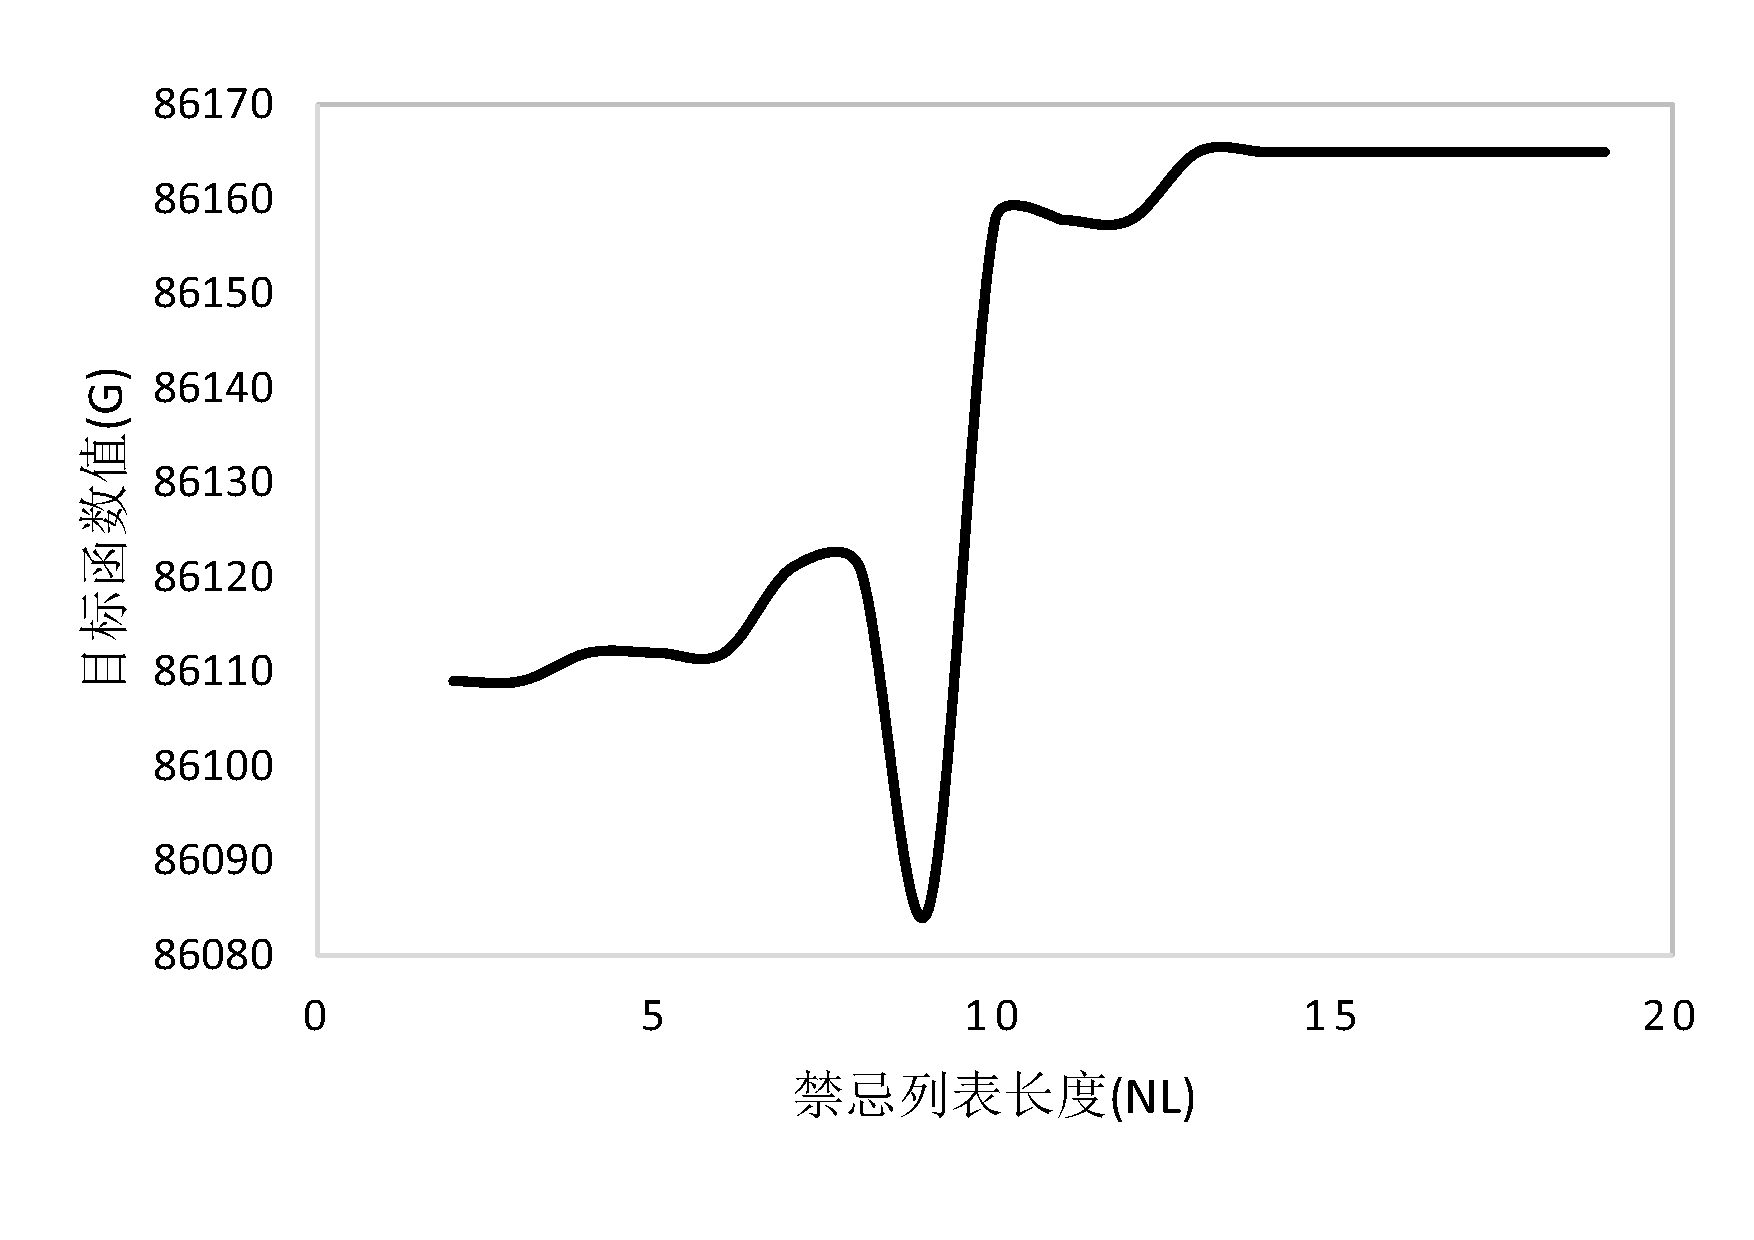
\includegraphics[height= 3.5cm,angle = -90]{NL_100}}
\subfloat[迭代次数]{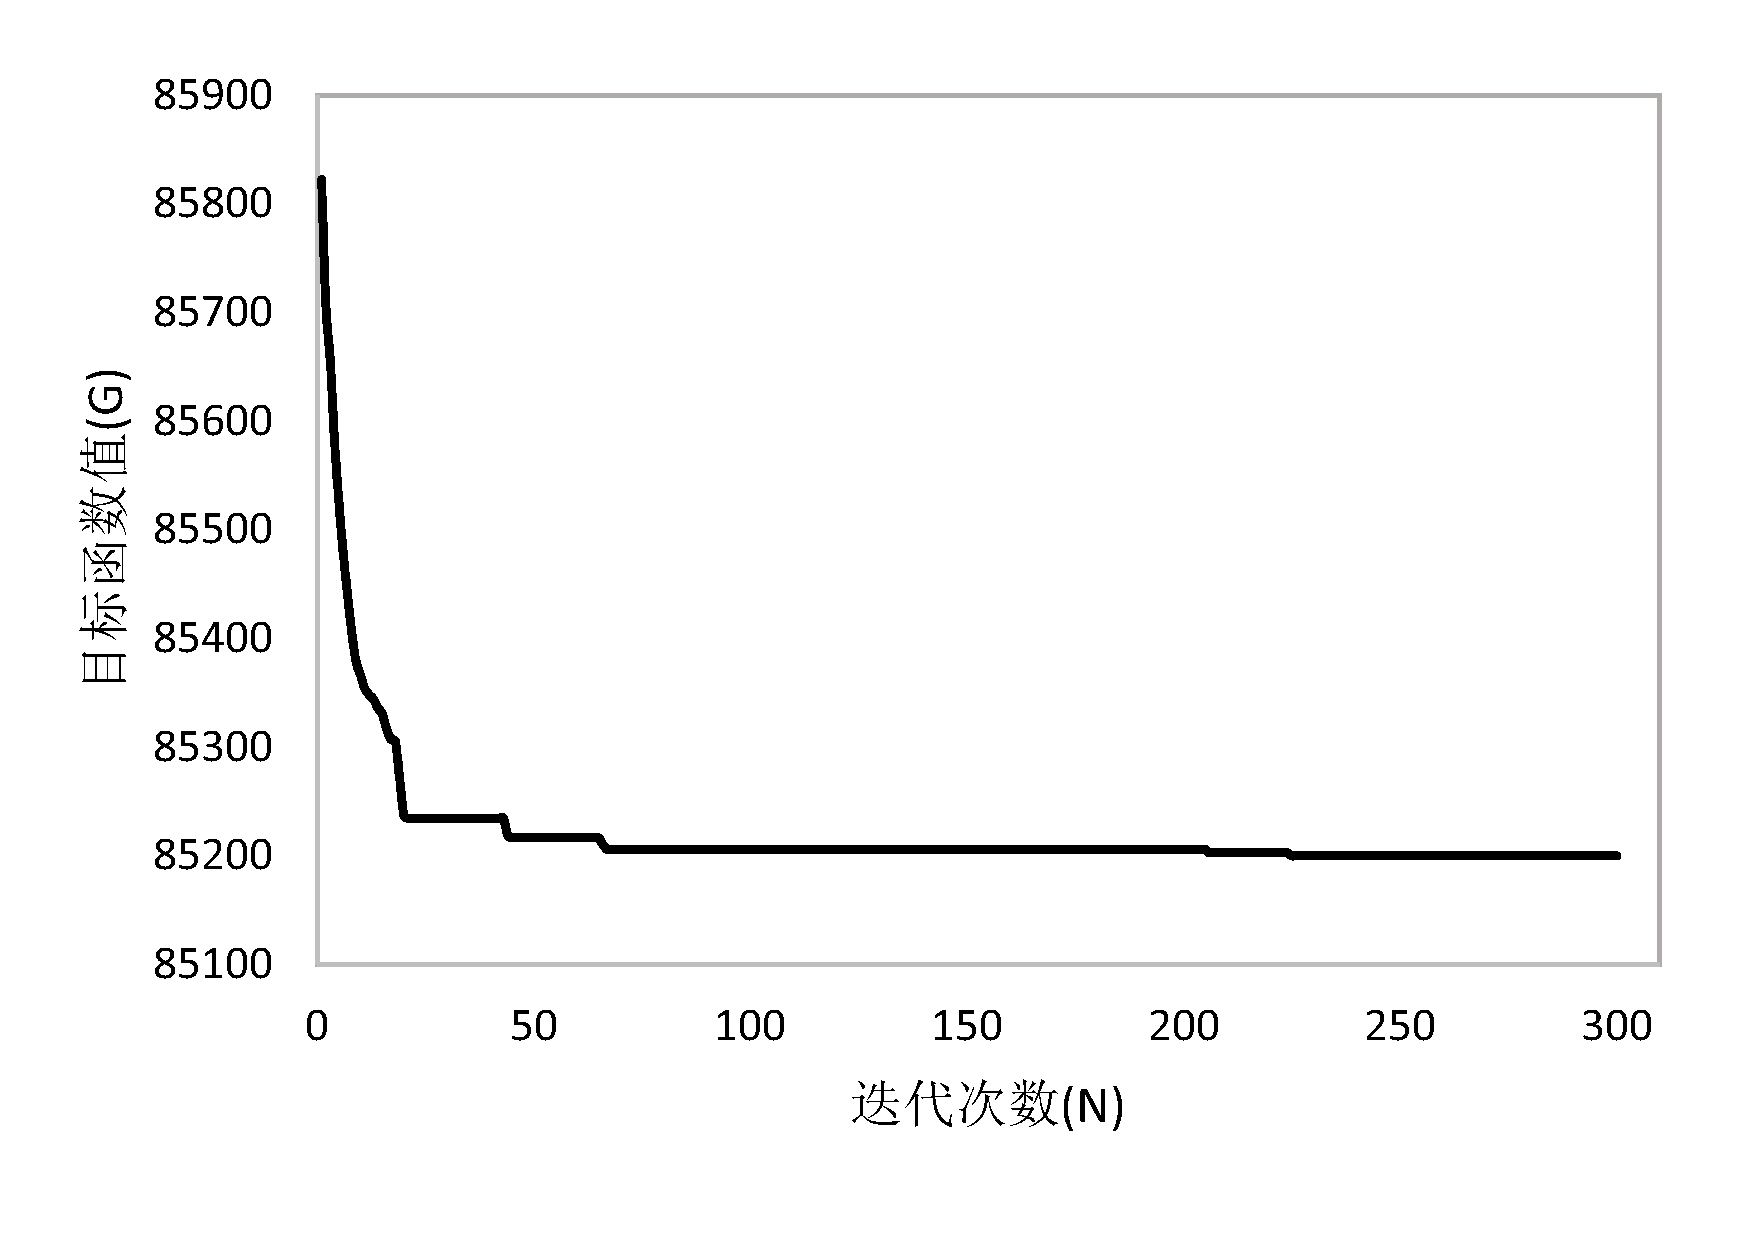
\includegraphics[height= 3.5cm,angle = -90]{N_100}}
\caption{$100$件订单的目标函数值和相关参数的关系}
\end{figure}
}
\onslide<2->{可以看出,$NL = 9$是最佳列表长度,取迭代次数$N = 70$是较为适宜的}
\transboxout<1->\end{frame}
\subsection{实验结果及评估}
\begin{frame}{实验结果示例}
\only<1>{以模型$1$ 为例,示例订单量$n = 20$,决策参数为$\lambda_1 = 0.6, \lambda_2 = 0.4$}
\only<2>{\begin{figure}
\centering
\resizebox{12cm}{!}{\begin{tikzpicture}
\fill[blue!20!] (101mm,2.5mm) rectangle (130mm,7.5mm) (79mm,22.5mm) rectangle (96mm,27.5mm) (77mm,32.5mm) rectangle (105mm,37.5mm) (110mm,32.5mm)rectangle(135mm,37.5mm) (95mm,42.5mm) rectangle (134mm,47.5mm) ;
\draw (70mm,-7mm) node{$G = 3978.8$};
\draw [->,very thick] (0,0) -- (140mm,0);
\draw (25mm,0) -- (25mm,1mm) (25mm,-3mm) node{$25$} (50mm,0) -- (50mm,1mm) (50mm,-3mm) node{$50$} (75mm,0) -- (75mm,1mm) (75mm,-3mm) node{$70$}  (100mm,0) -- (100mm,1mm) (100mm,-3mm) node{$100$} (125mm,0) -- (125mm,1mm) (125mm,-3mm) node{$125$} (143mm,0) node{$tu$};
\draw [very thick] (0,0) -- (0,50mm) (0.4,53mm) node{流水线};
\draw [thick] (-2mm,5mm) node{$1$} (0,2.5mm) rectangle (24mm,7.5mm) rectangle (62mm,2.5mm) rectangle (101mm,7.5mm) rectangle (130mm,2.5mm);
\draw [thick] (-2mm,15mm) node{$2$} (0,12.5mm) rectangle (37mm,17.5mm) rectangle (63mm,12.5mm) rectangle (104mm,17.5mm);
\draw [thick] (-2mm,25mm) node{$3$} (0,22.5mm) rectangle (27mm,27.5mm) rectangle (62mm,22.5mm) rectangle (79mm,27.5mm) rectangle (96mm,22.5mm) ;
\draw [thick] (-2mm,35mm) node{$4$} (0,32.5mm) rectangle (27mm,37.5mm) rectangle (56mm,32.5mm) rectangle (77mm,37.5mm) rectangle (105mm,32.5mm) rectangle(135mm,37.5mm);
\draw [thick] (-2mm,45mm) node{$5$} (0,42.5mm) rectangle (22mm,47.5mm) rectangle (52mm,42.5mm) rectangle (95mm,47.5mm) rectangle (134mm, 42.5mm);
\draw (11mm,45mm) node{$5$} (37mm,45mm) node{$1$} (73.5mm,45mm) node{$3$} (114.5mm,45mm) node{$19$} ;
\draw (13.5mm,35mm) node{$4$} (41.5mm,35mm) node{$8$} (66.5mm,35mm) node{$17$} (91mm,35mm) node{$12$} (120mm,35mm) node{$20$};
\draw (13.5mm,25mm) node{$16$} (44.5mm,25mm) node{$15$} (70.5mm,25mm) node{$13$} (87.5mm,25mm) node{$9$};
\draw (18.5mm,15mm) node{$11$} (50mm,15mm) node{$7$} (83.5mm,15mm) node{$2$} ;
\draw (12mm,5mm) node{$10$} (43mm,5mm) node{$18$} (79.5mm,5mm) node{$14$} (115.5mm,5mm) node{$6$};
\end{tikzpicture}}
\caption{Cyc -- ATC 算法调度结果}
\end{figure}}
\only<3>{\begin{figure}
\centering
\resizebox{12cm}{!}{\begin{tikzpicture}
\fill[blue!20!] (112mm,2.5mm) rectangle (130mm,7.5mm) (116mm,12.5mm) rectangle (134mm,17.5mm) (77mm,32.5mm) rectangle (105mm,37.5mm) (98mm,42.5mm) rectangle (134mm,47.5mm) ;
\draw [->,very thick] (0,0) -- (140mm,0);
\draw (25mm,0) -- (25mm,1mm) (25mm,-3mm) node{$25$} (50mm,0) -- (50mm,1mm) (50mm,-3mm) node{$50$} (75mm,0) -- (75mm,1mm) (75mm,-3mm) node{$70$}  (100mm,0) -- (100mm,1mm) (100mm,-3mm) node{$100$} (125mm,0) -- (125mm,1mm) (125mm,-3mm) node{$125$} (143mm,0) node{$tu$};
\draw (70mm,-7mm) node{$G = 3478.8$};
\draw [very thick] (0,0) -- (0,50mm) (0.4,53mm) node{流水线};
\draw [thick] (-2mm,5mm) node{$1$} (0,2.5mm) rectangle (24mm,7.5mm) rectangle (53mm,2.5mm) rectangle (91mm,7.5mm) rectangle (130mm,2.5mm);
\draw [thick] (-2mm,15mm) node{$2$} (0,12.5mm) rectangle (26mm,17.5mm) rectangle (63mm,12.5mm) rectangle (93mm,17.5mm) rectangle (134mm,12.5mm);
\draw [thick] (-2mm,25mm) node{$3$} (0,22.5mm) rectangle (17mm,27.5mm) rectangle (34mm,22.5mm) rectangle (61mm,27.5mm) rectangle (96mm,22.5mm) ;
\draw [thick] (-2mm,35mm) node{$4$} (0,32.5mm) rectangle (27mm,37.5mm) rectangle (56mm,32.5mm) rectangle (77mm,37.5mm) rectangle (105mm,32.5mm);
\draw [thick] (-2mm,45mm) node{$5$} (0,42.5mm) rectangle (22mm,47.5mm) rectangle (61mm,42.5mm) rectangle (91mm,47.5mm) rectangle (134mm, 42.5mm);
\draw (11mm,45mm) node{$5$} (41.5mm,45mm) node{$19$} (76mm,45mm) node{$1$} (112.5mm,45mm) node{$3$} ;
\draw (13.5mm,35mm) node{$4$} (41.5mm,35mm) node{$8$} (66.5mm,35mm) node{$17$} (91mm,35mm) node{$12$} ;
\draw (8.5mm,25mm) node{$9$} (25.5mm,25mm) node{$13$} (47.5mm,25mm) node{$16$} (78.5mm,25mm) node{$15$};
\draw (13mm,15mm) node{$7$} (44.5mm,15mm) node{$11$} (78mm,15mm) node{$20$} (113.5mm,15mm) node{$2$};
\draw (12mm,5mm) node{$10$} (38.5mm,5mm) node{$6$} (72mm,5mm) node{$18$} (110.5mm,5mm) node{$14$} ;
\end{tikzpicture}}
\caption{Cyc -- Tabu 算法调度结果}
\end{figure}}
\only<4>{\begin{figure}
\centering
\resizebox{12cm}{!}{\begin{tikzpicture}
\fill[blue!20!] (91mm,2.5mm) rectangle (92mm,7.5mm) (116mm,2.5mm) rectangle (133mm,7.5mm) (99mm,22.5mm) rectangle (125mm,27.5mm) (98mm,32.5mm) rectangle (127mm,37.5mm) (96mm,42.5mm) rectangle (112mm,47.5mm) ;
\draw [->,very thick] (0,0) -- (140mm,0);
\draw (25mm,0) -- (25mm,1mm) (25mm,-3mm) node{$25$} (50mm,0) -- (50mm,1mm) (50mm,-3mm) node{$50$} (75mm,0) -- (75mm,1mm) (75mm,-3mm) node{$70$}  (100mm,0) -- (100mm,1mm) (100mm,-3mm) node{$100$} (125mm,0) -- (125mm,1mm) (125mm,-3mm) node{$125$} (143mm,0) node{$tu$};
\draw (70mm,-7mm) node{$G = 3329.2$};
\draw [very thick] (0,0) -- (0,50mm) (0.4,53mm) node{流水线};
\draw [thick] (-2mm,5mm) node{$1$} (0,2.5mm) rectangle (24mm,7.5mm) rectangle (54mm,2.5mm) rectangle (92mm,7.5mm) rectangle (133mm,2.5mm);
\draw [thick] (-2mm,15mm) node{$2$} (0,12.5mm) rectangle (26mm,17.5mm) rectangle (63mm,12.5mm) rectangle (102mm,17.5mm);
\draw [thick] (-2mm,25mm) node{$3$} (0,22.5mm) rectangle (17mm,27.5mm) rectangle (34mm,22.5mm) rectangle (61mm,27.5mm) rectangle (96mm,22.5mm) rectangle (125mm,27.5mm);
\draw [thick] (-2mm,35mm) node{$4$} (0,32.5mm) rectangle (27mm,37.5mm) rectangle (56mm,32.5mm) rectangle (99mm,37.5mm) rectangle (127mm,32.5mm);
\draw [thick] (-2mm,45mm) node{$5$} (0,42.5mm) rectangle (22mm,47.5mm) rectangle (61mm,42.5mm) rectangle (91mm,47.5mm) rectangle (112mm, 42.5mm);
\draw (11mm,45mm) node{$5$} (41.5mm,45mm) node{$19$} (76mm,45mm) node{$1$} (101.5mm,45mm) node{$17$} ;
\draw (13.5mm,35mm) node{$4$} (41.5mm,35mm) node{$8$} (77.5mm,35mm) node{$3$} (113mm,35mm) node{$12$} ;
\draw (8.5mm,25mm) node{$9$} (25.5mm,25mm) node{$13$} (47.5mm,25mm) node{$16$} (78.5mm,25mm) node{$15$} (110.5mm,25mm) node{$6$};
\draw (13mm,15mm) node{$7$} (44.5mm,15mm) node{$11$} (82.5mm,15mm) node{$14$} ;
\draw (12mm,5mm) node{$10$} (39mm,5mm) node{$20$} (73mm,5mm) node{$18$} (112.5mm,5mm) node{$2$};
\end{tikzpicture}}
\caption{Vtr -- Tabu 算法调度结果}
\end{figure}}
\transboxout<1->\end{frame}

\begin{frame}{模型1求解结果与分析}{不同决策环境分析}
\onslide<1->{以$m = 6, n = 200$为例}
\onslide<2->{\begin{figure}
\centering
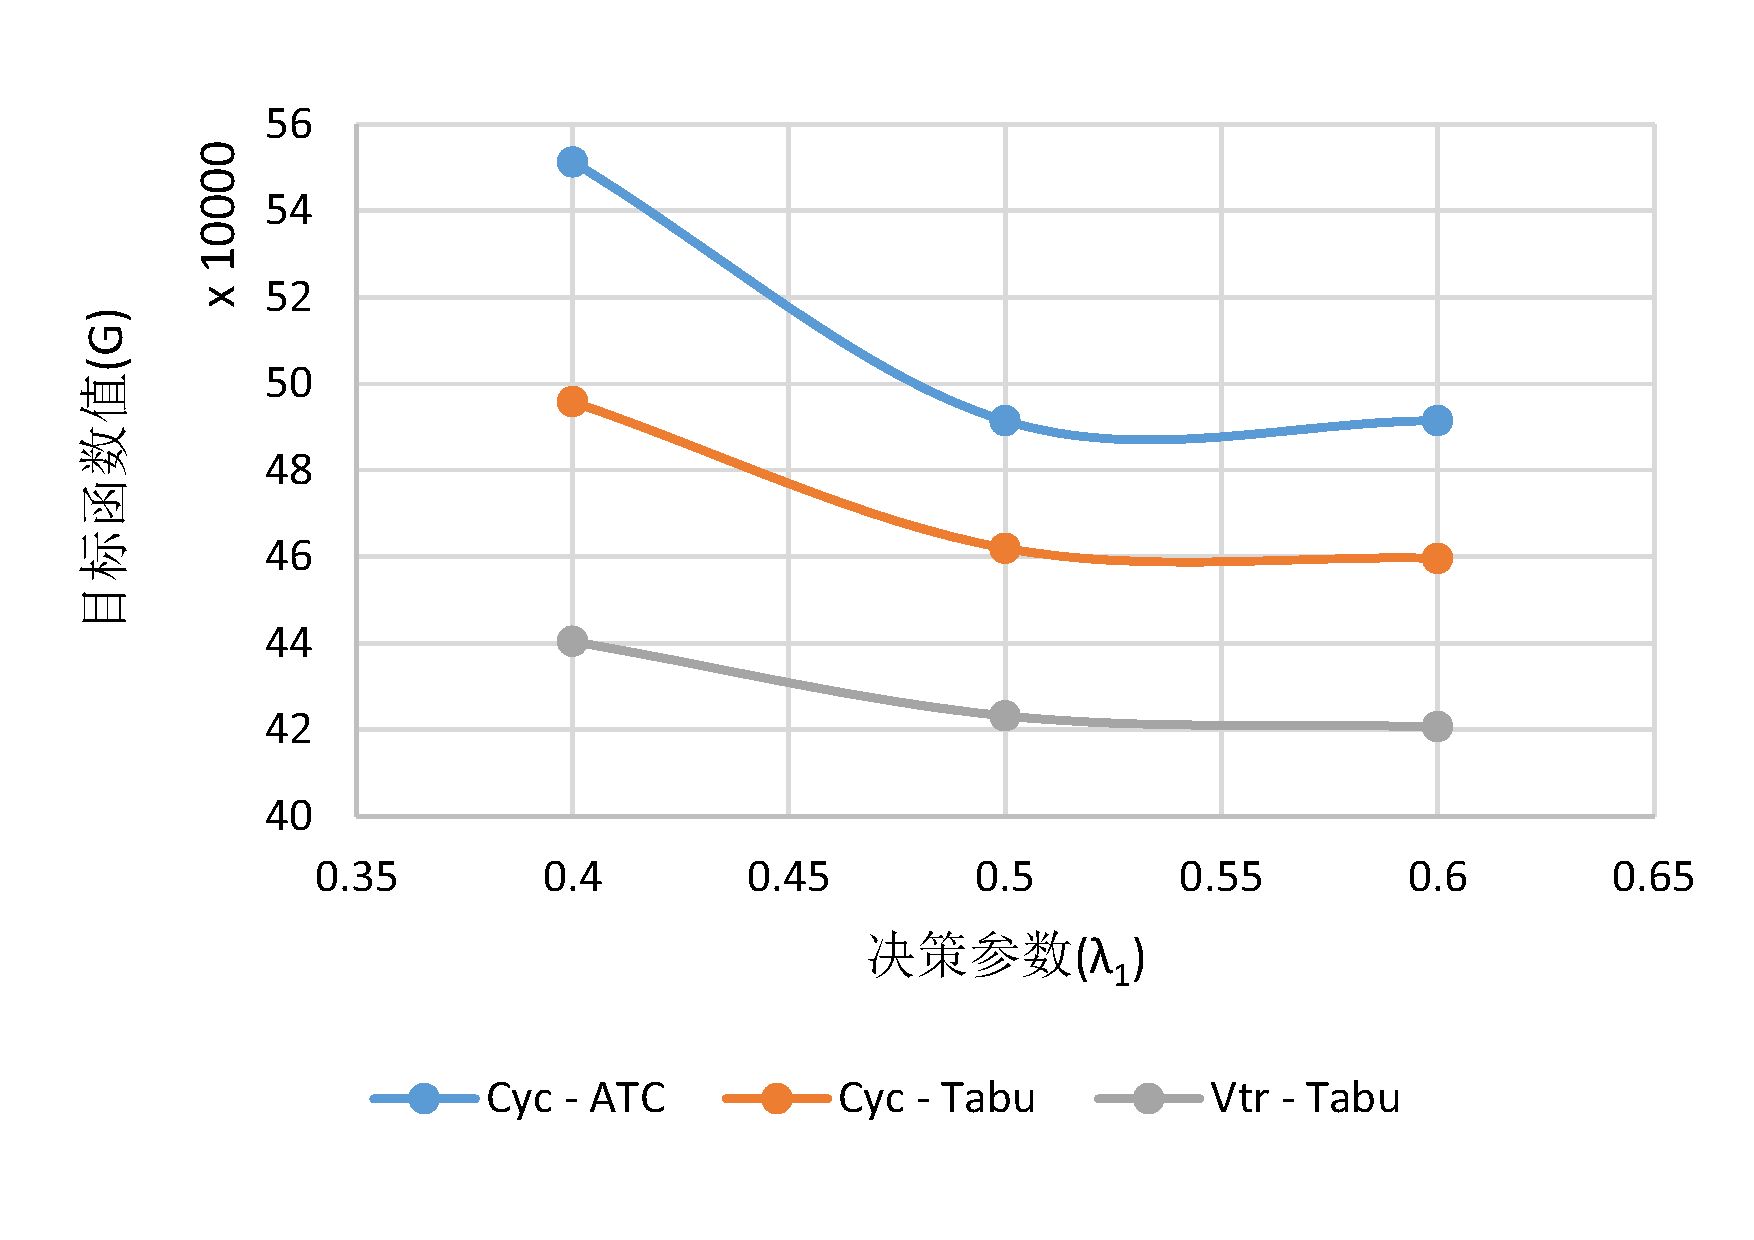
\includegraphics[height = 6cm, angle = -90]{lambda.pdf}
\caption{决策参数和目标函数值关系示例}
\end{figure}}
\transboxout<1->\end{frame}
\begin{frame}{模型2求解结果与分析}{流水线均衡率分析}
\begin{figure}[h]
\centering
\subfloat[$m = 5$]{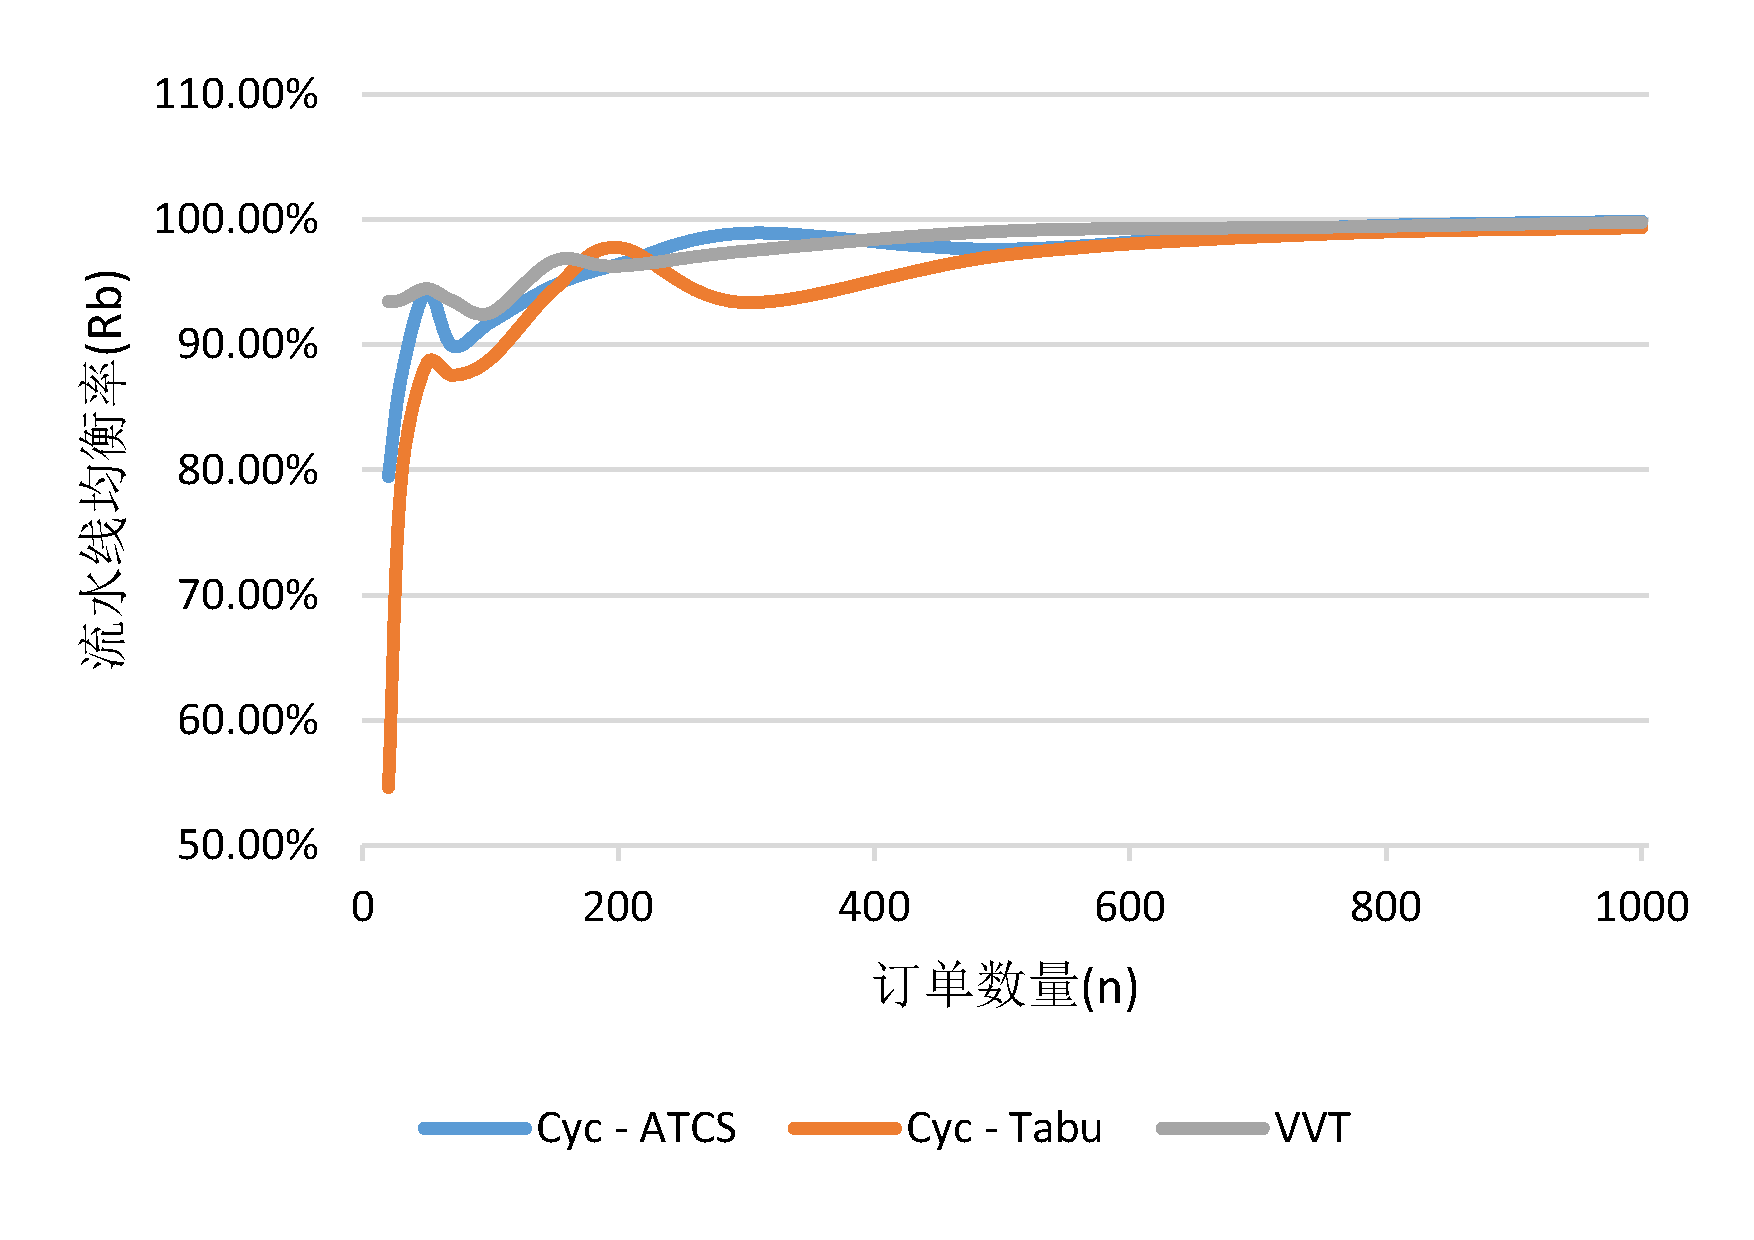
\includegraphics[height = 4cm,angle = -90]{rb_05_5.pdf}}
\subfloat[$m = 6$]{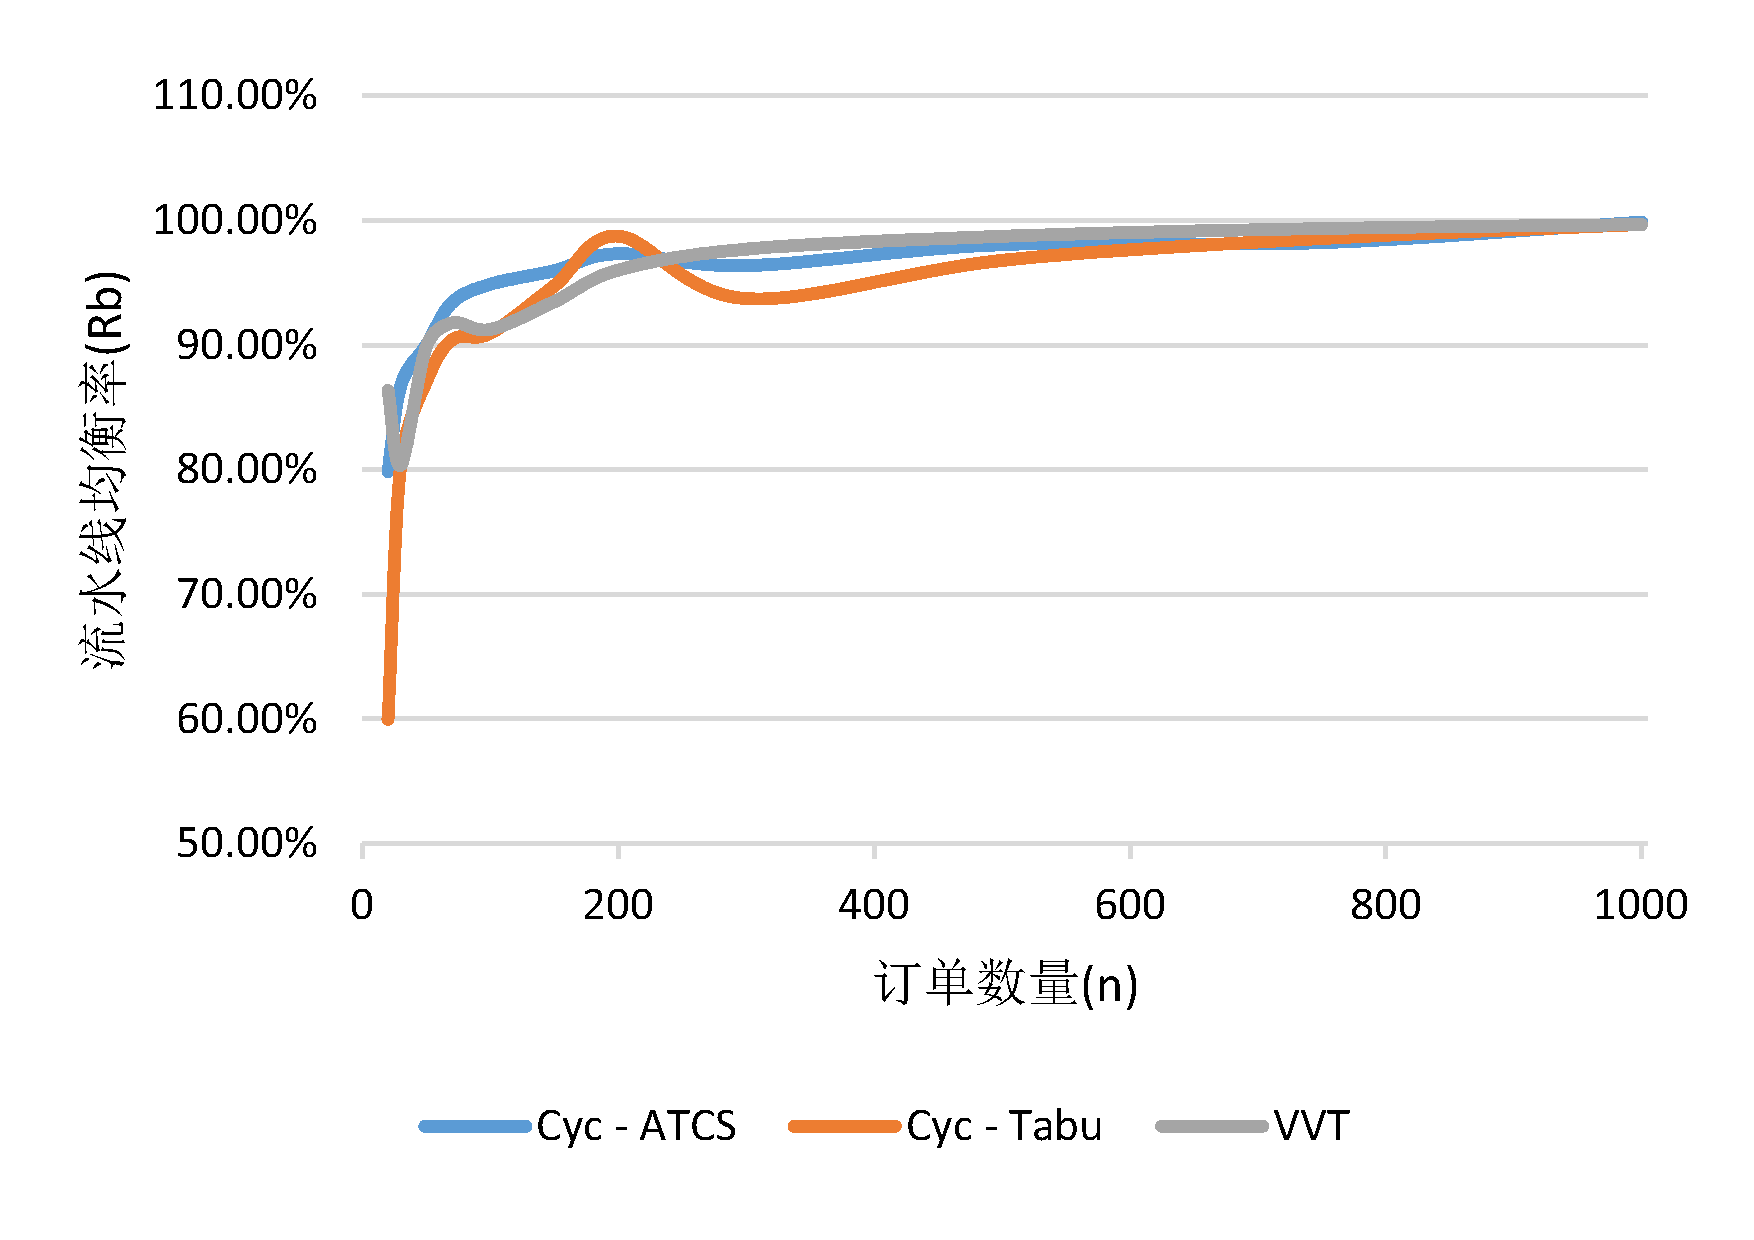
\includegraphics[height = 4cm,angle = -90]{rb_05_6.pdf}}
\subfloat[$m = 7$]{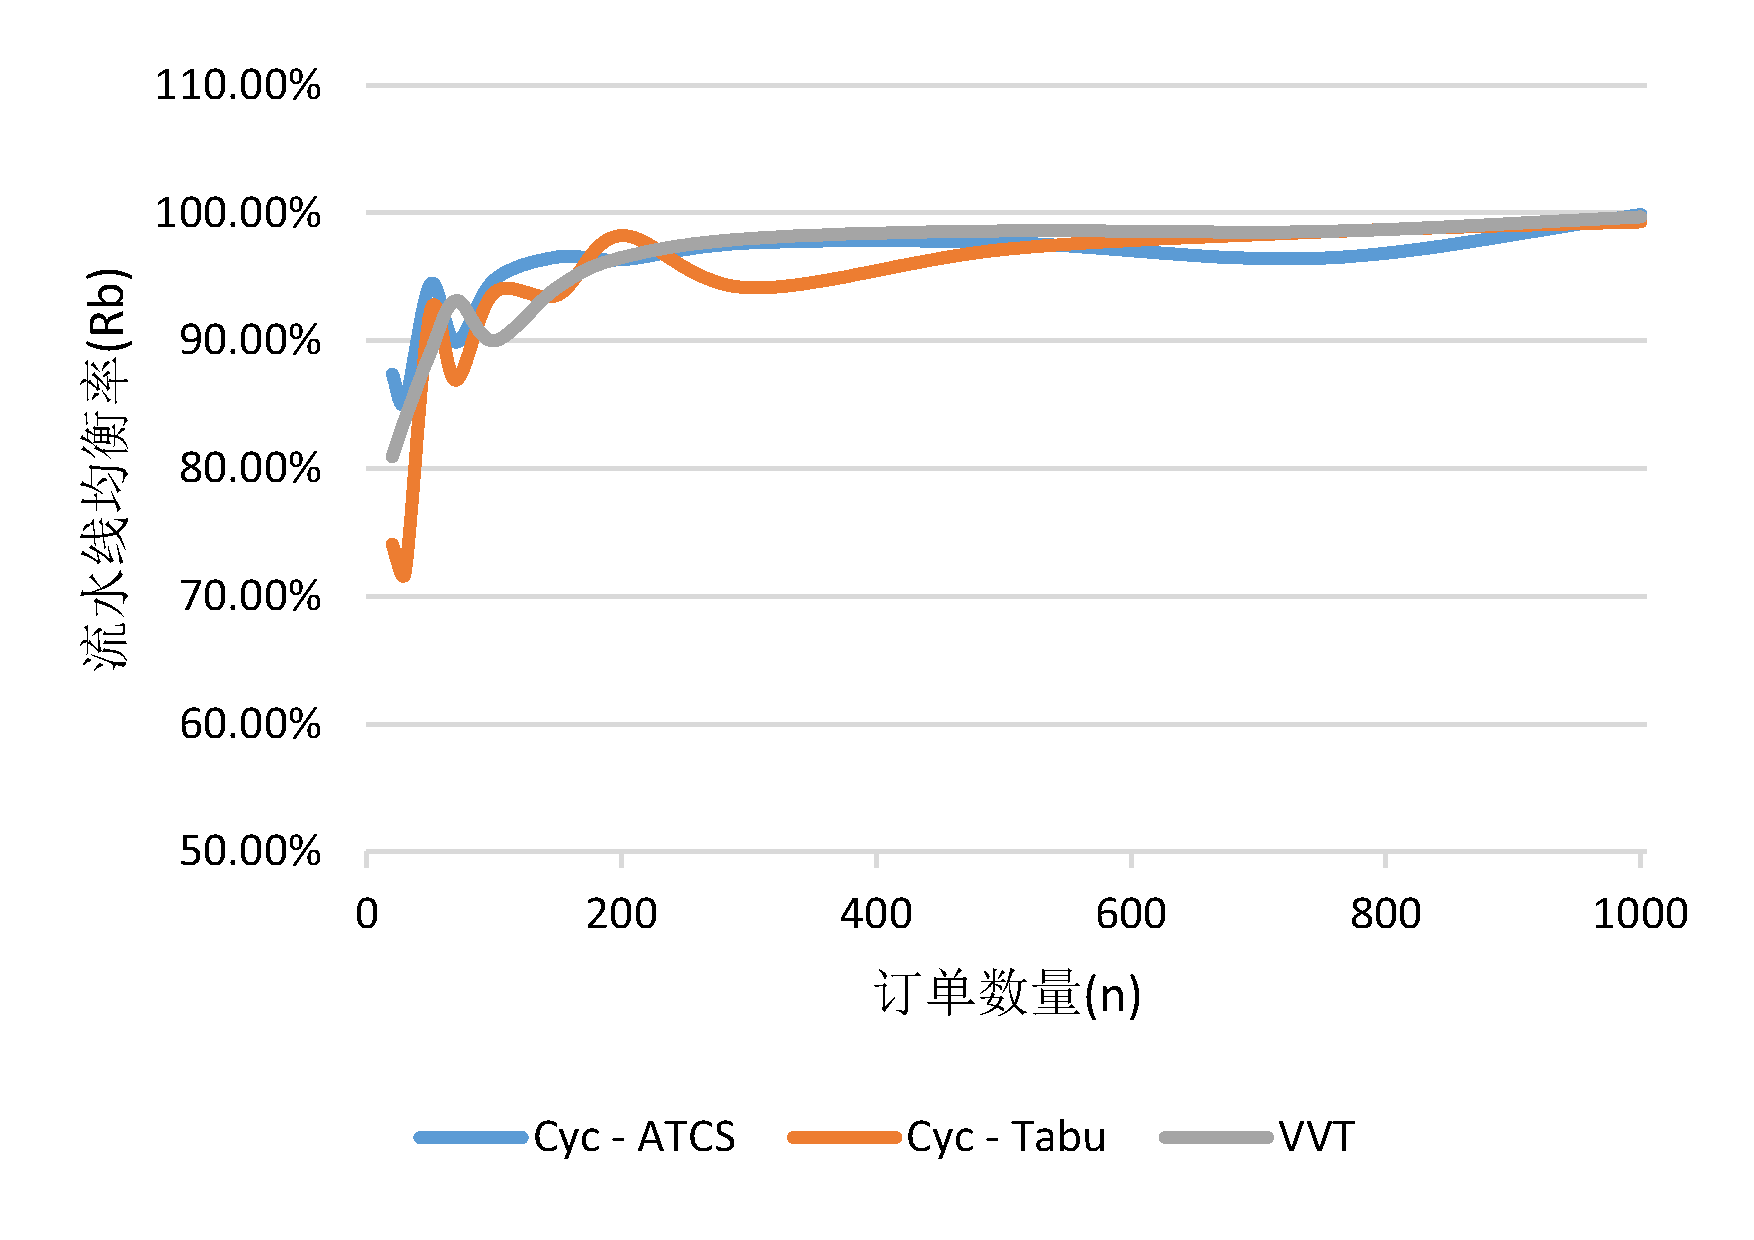
\includegraphics[height = 4cm,angle = -90]{rb_05_7.pdf}}
\caption{不同流水线数量和流水线均衡率关系($\lambda_1 = 0.5$)}
\end{figure}
\transboxout<1->\end{frame}
\begin{frame}{模型2求解结果与分析}{不同决策环境分析}
\begin{figure}
\centering
\subfloat[$\lambda_1= 0.4$]{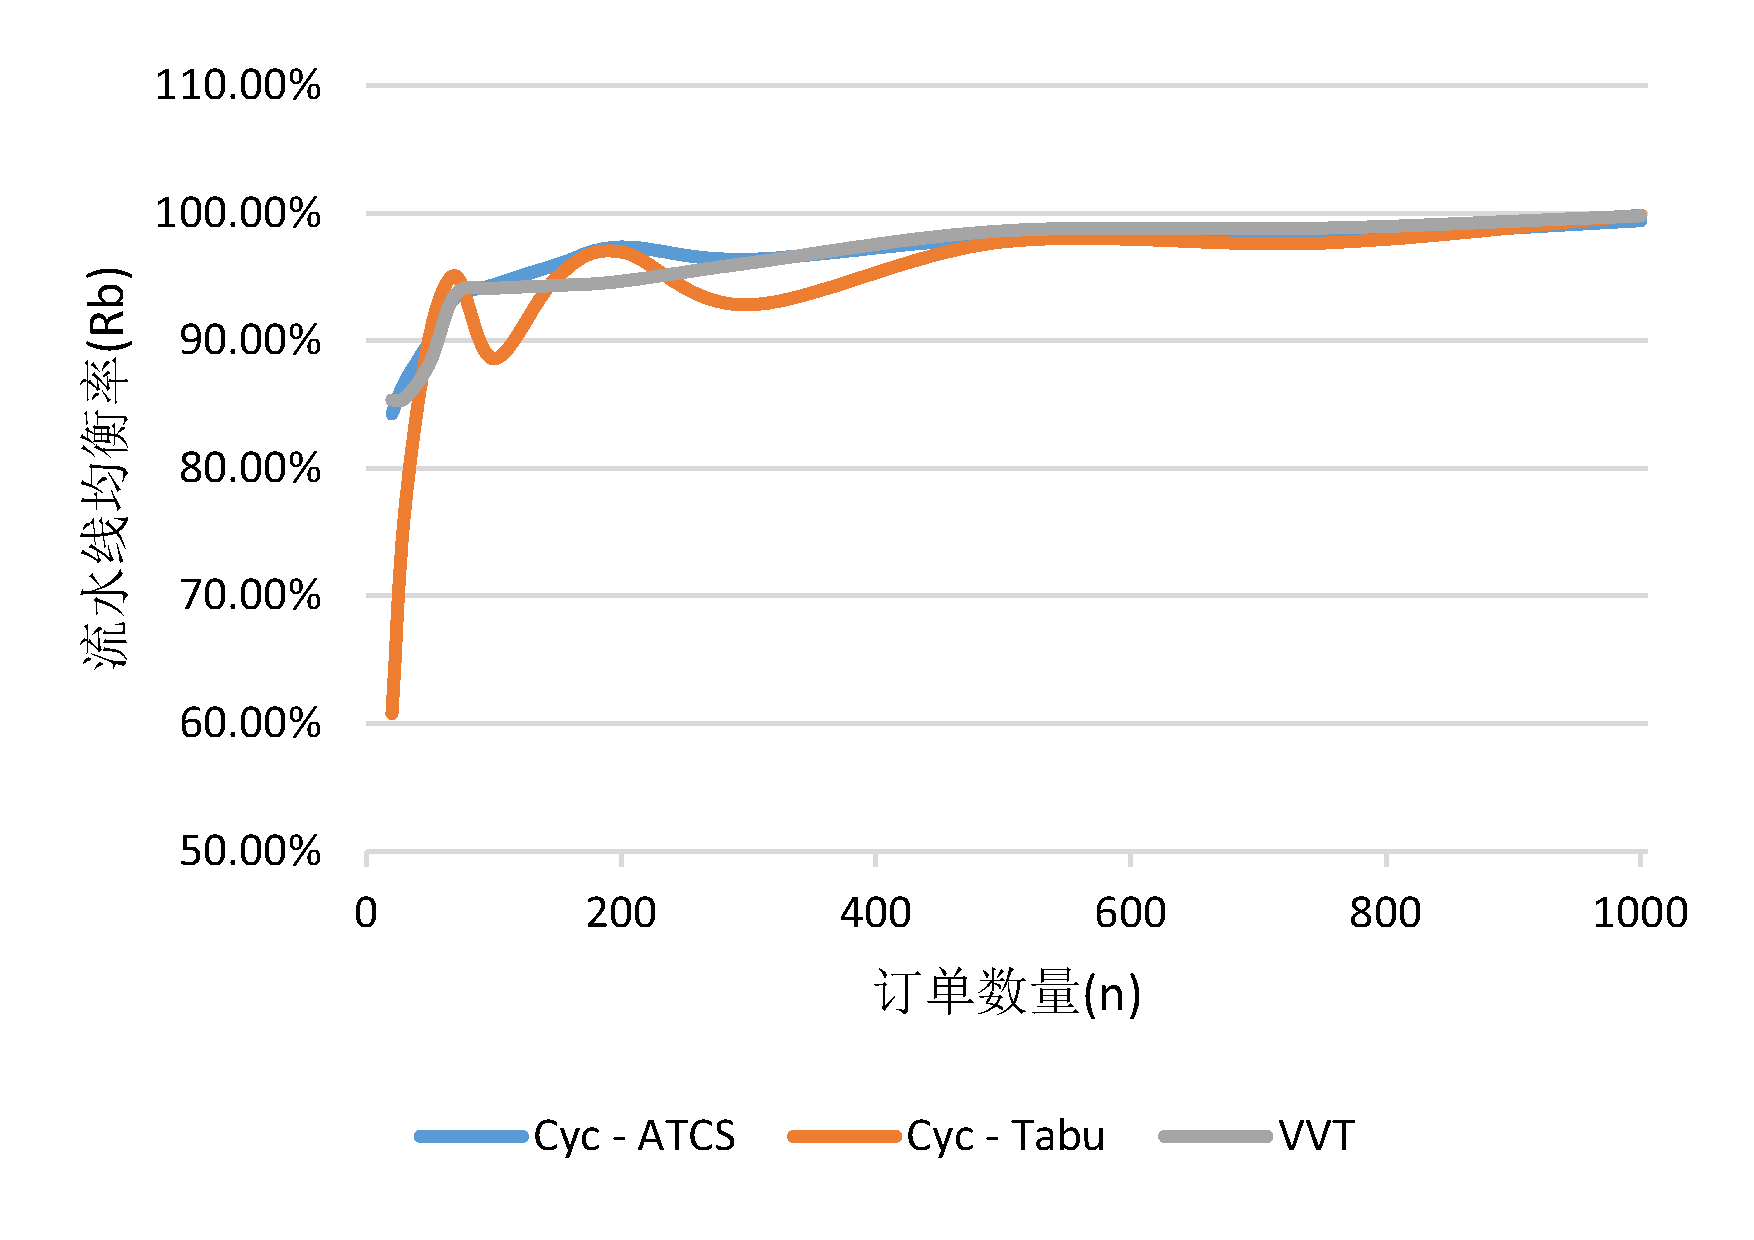
\includegraphics[height = 5.6cm,angle = -90]{rb_04_6.pdf}}
\subfloat[$\lambda_1= 0.6$]{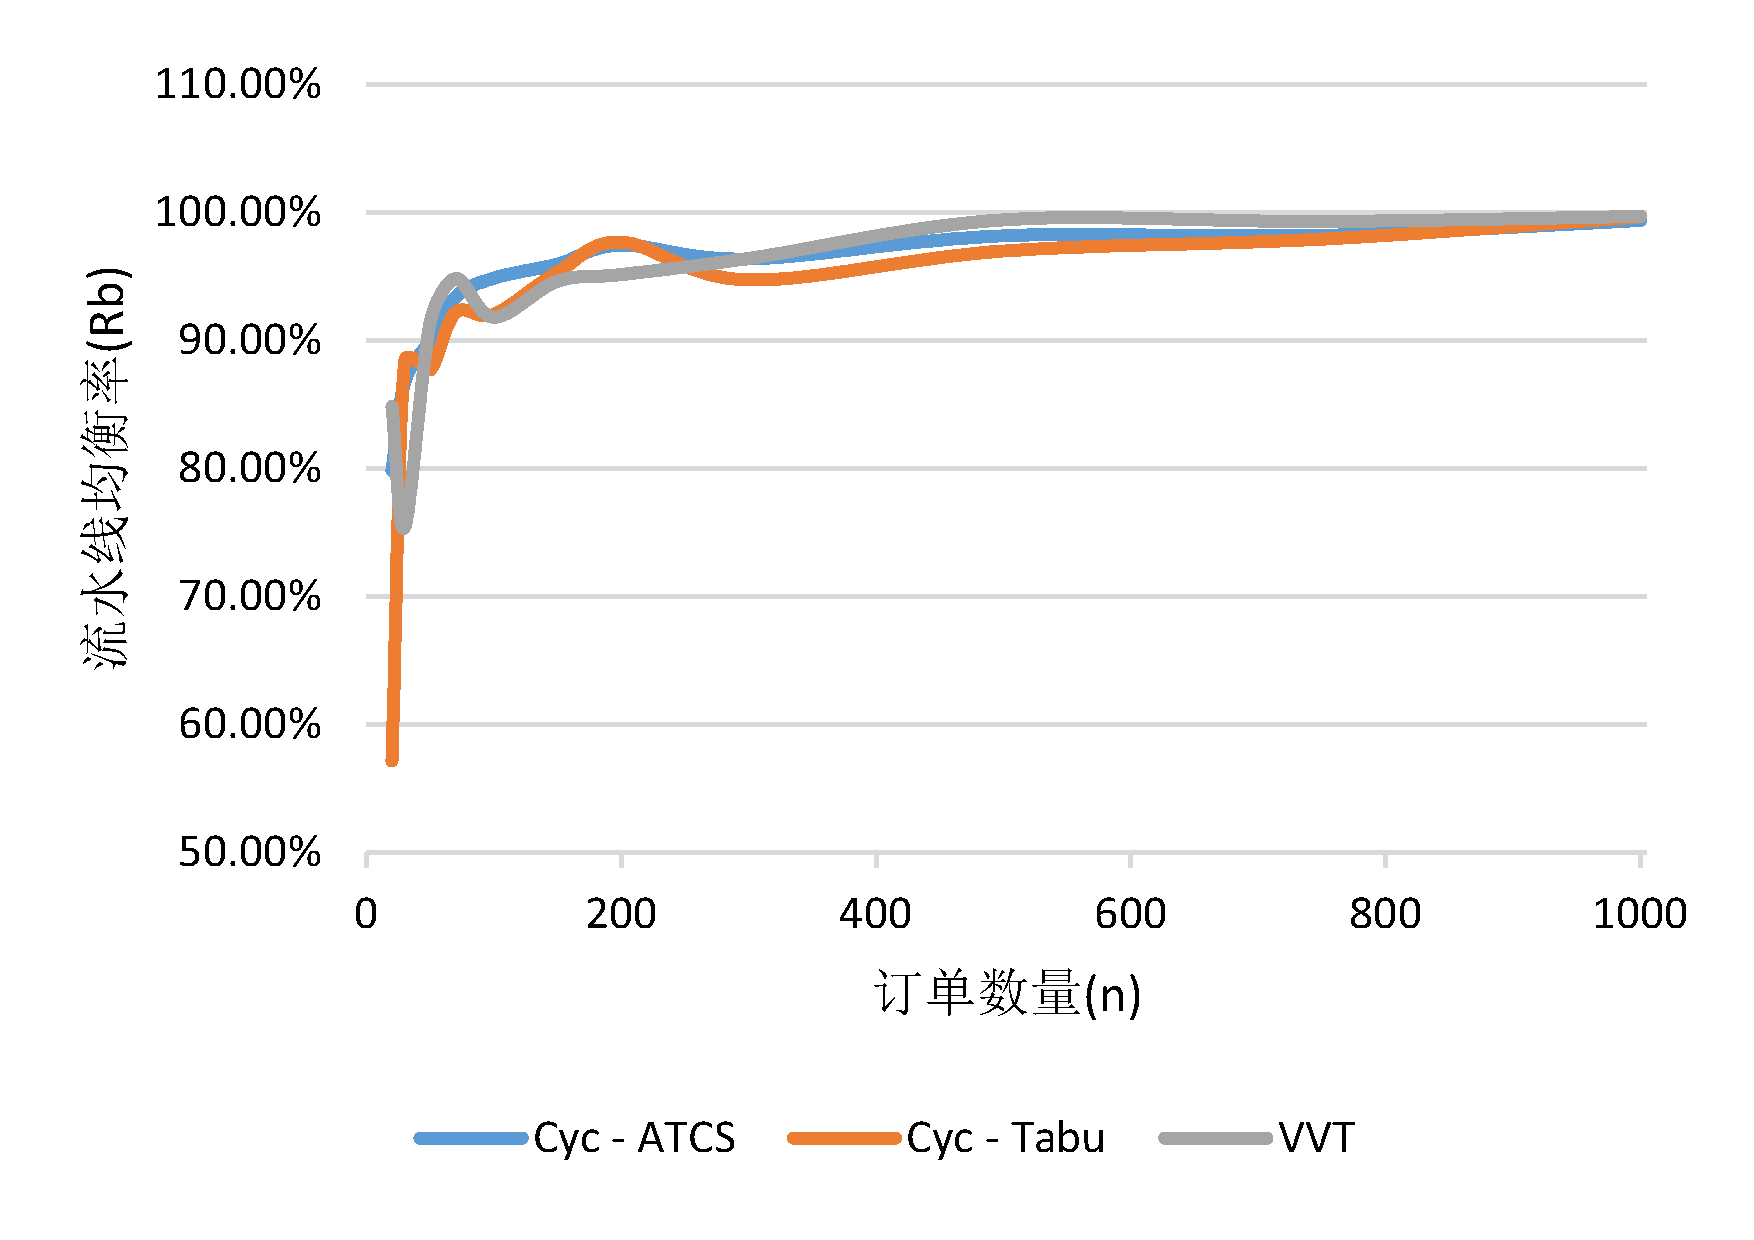
\includegraphics[height = 5.6cm,angle = -90]{rb_06_6.pdf}}
\caption{决策环境和流水线均衡率关系$(m = 6)$}
\end{figure}
\transboxout<1->\end{frame}
\section{ }
\begin{frame}
\centering
\Huge
谢~~谢!
\transboxout<1->\end{frame}
\end{document}